\newpage
\section{Phân tích thiết kế hệ thống}


\subsection{Bài toán nghiệp vụ}

Hệ thống hỗ trợ người dùng
hỏi đáp pháp luật Việt Nam,
phân tích tài liệu
và đàm thoại trực tiếp thời gian thực
với trợ lý ảo pháp lý.
Dựa trên thiết kế hướng miền (DDD),
bài toán lớn được chia làm
các miền phụ (Subdomain)
với các chức năng như sau:


\begin{figure}[H]
\centering
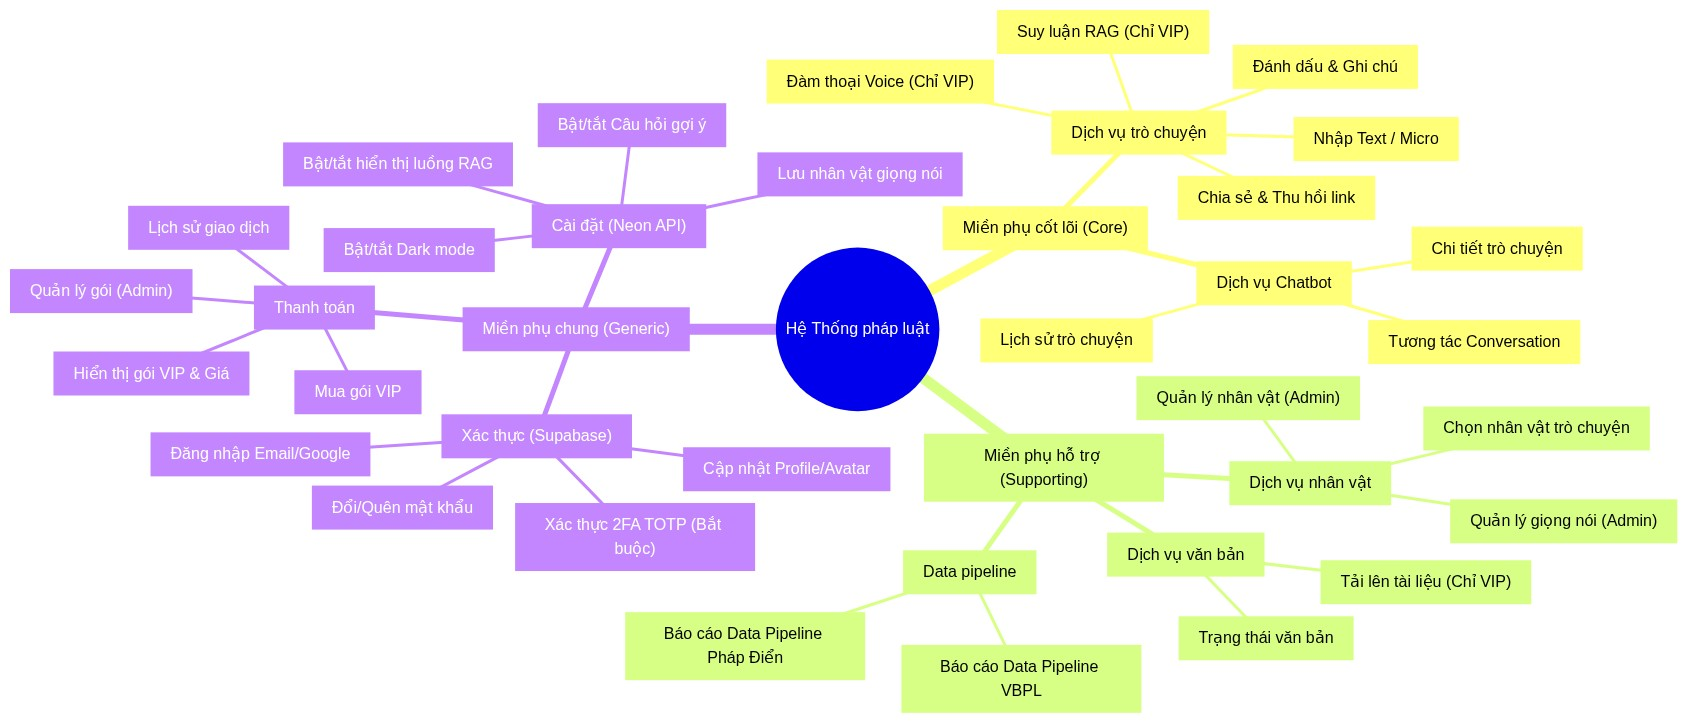
\includegraphics[scale = 0.25]{pictures/SubDomain.png}
\caption{Sơ đồ tổng quan SubDomain}
\end{figure}


\subsubsection{Miền phụ cốt lõi (Core Subdomain)}

Miền phụ cốt lõi
là phần quan trọng
và có giá trị nhất của hệ thống.
Miền phụ cốt lõi
giúp phân biệt các doanh nghiệp
và làm cho các doanh nghiệp có giá trị.
Miền phụ cốt lõi
tập trung vào mục tiêu
và yêu cầu của khách hàng với doanh nghiệp,
từ đó quyết định sự thành công của doanh nghiệp.
Vì vậy, mỗi doanh nghiệp
luôn tìm cách thực hiện những điều khác biệt
trong các miền phụ cốt lõi này để đạt được lợi thế so với đối thủ cạnh tranh.


\begin{itemize}


\item Dịch vụ trò chuyện (conversation service)


\begin{itemize}


\item Nhập văn bản bằng text hoặc micro
\item Chức năng đàm thoại giọng nói Voice (Chỉ dành cho người dùng đã thanh toán VIP)
\item Sử dụng chức năng RAG suy luận (Chỉ dành cho người dùng đã thanh toán VIP)
\item Đánh dấu cuộc trò chuyện theo thư mục và ghi chú
\item Tạo liên kết chia sẻ và thu hồi cuộc trò chuyện

\end{itemize}


\item Dịch vụ chatbot (chatbot service)


\begin{itemize}


\item Tương tác giao tiếp với conversation service
\item Tương tác giao tiếp với livekit server
\item Lấy thông tin về lịch sử trò chuyện
\item Lấy thông tin chi tiết trò chuyện
\end{itemize}

\end{itemize}


Miền phụ cốt lõi
là nơi diễn ra các luồng xử lý phức tạp
và quyết định đến mức độ hài lòng của người dùng.


\subsubsection{Miền phụ hỗ trợ (Supporting Subdomain)}

Các miền phụ cốt lõi phụ thuộc
vào các miền phụ hỗ trợ.
Miền phụ hỗ trợ cung cấp các dịch vụ
để miền phụ cốt lõi hoạt động hiệu quả.
Tuy nhiên, miền phụ hỗ trợ không đòi hỏi mức độ phức tạp cao về logic nghiệp vụ.


\begin{itemize}


\item Dịch vụ văn bản (document service)
\begin{itemize}
\item Tải lên file tài liệu văn bản (Chỉ dành cho người dùng đã thanh toán VIP)
\item Lấy thông tin trạng thái văn bản
\end{itemize}
\item Dịch vụ nhân vật (persona service)
\begin{itemize}
\item Người dùng lựa chọn nhân vật để trò chuyện giọng nói
\item Quản lý nhân vật (cần vai trò ADMIN)
\item Quản lý giọng nói (cần vai trò ADMIN)
\end{itemize}
\item Báo cáo Data pipeline
\begin{itemize}
\item Báo cáo thông tin Data pipeline của văn bản pháp luật
\item Báo cáo thông tin Data pipeline của Pháp Điển
\end{itemize}


\end{itemize}


Miền phụ hỗ trợ giúp miền phụ cốt lõi không bị phình to.
Tách nhỏ việc quản lý nhân vật, giọng nói
và quá trình xử lý tài liệu tiêu tốn nhiều tài nguyên hệ thống.

\subsubsection{Miền phụ chung (Generic Subdomain)}

Miền phụ chung
cung cấp các giải pháp có sẵn
mà doanh nghiệp có thể mua, thuê.
Miền phụ chung
có thể được tìm thấy trên nhiều ngành.
Doanh nghiệp không thể đạt được bất kỳ lợi thế cạnh tranh so
với đối thủ bằng cách thực hiện những điều khác biệt trong miền phụ chung.


\begin{itemize}


\item Dịch vụ xác thực (auth service - dùng supabase)
\begin{itemize}
\item Người dùng đăng ký, đăng nhập bằng email hoặc đăng nhập bằng Google
\item Người dùng xem thông tin cá nhân và cập nhật tên, cập nhật ảnh avatar
\item Người dùng có thể đổi mật khẩu hoặc dùng quên mật khẩu
\item Xác thực 2FA bằng TOTP (bắt buộc vì dữ liệu pháp luật cần bảo mật)
\end{itemize}
\item Dịch vụ cài đặt (setting service - dùng neon api)
\begin{itemize}
\item Lưu thông tin nhân vật giọng nói
\item Bật tắt giao diện Dark mode
\item Bật tắt câu hỏi gợi ý
\item Bật tắt Tự động hiển thị các bước suy luận RAG trong cuộc trò chuyện
\end{itemize}
\item Dịch vụ thanh toán (payment service)
\begin{itemize}
\item Hiển thị các gói VIP và mức giá
\item Quản lý các gói (cần vai trò ADMIN)
\item Người dùng mua gói VIP để nâng cấp tài khoản
\item Lưu lịch sử giao dịch


\end{itemize}
\end{itemize}


Việc áp dụng các giải pháp có sẵn
như Supabase (Auth) hay Neon API (Settings)
là một chiến lược thông minh
để rút ngắn thời gian phát triển.
Đặc biệt là việc tích hợp 2FA,
điều kiện tiên quyết
cho các hệ thống xử lý hợp đồng
và dữ liệu pháp luật mang tính nhạy cảm.


Sơ đồ phân rã chức năng


\begin{figure}[H]
\centering
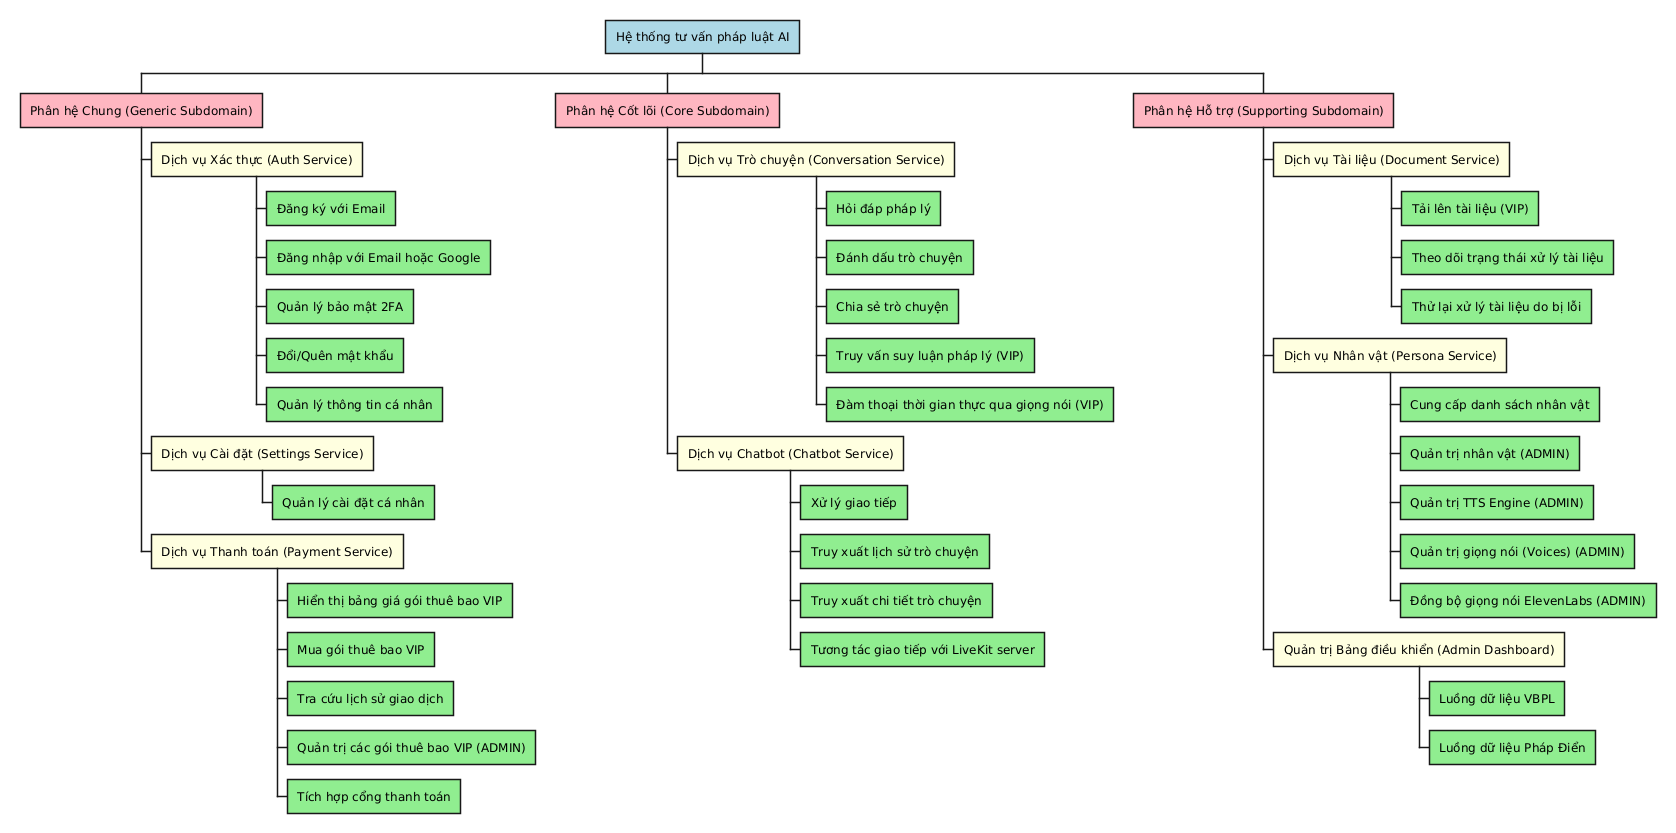
\includegraphics[scale = 0.18]{pictures/BFD.png}
\caption{Sơ đồ phân rã chức năng}
\end{figure}


\subsection{Phân tích thiết kế hệ thống}


\subsubsection{Sơ đồ Use Case}


\begin{figure}[H]
\centering
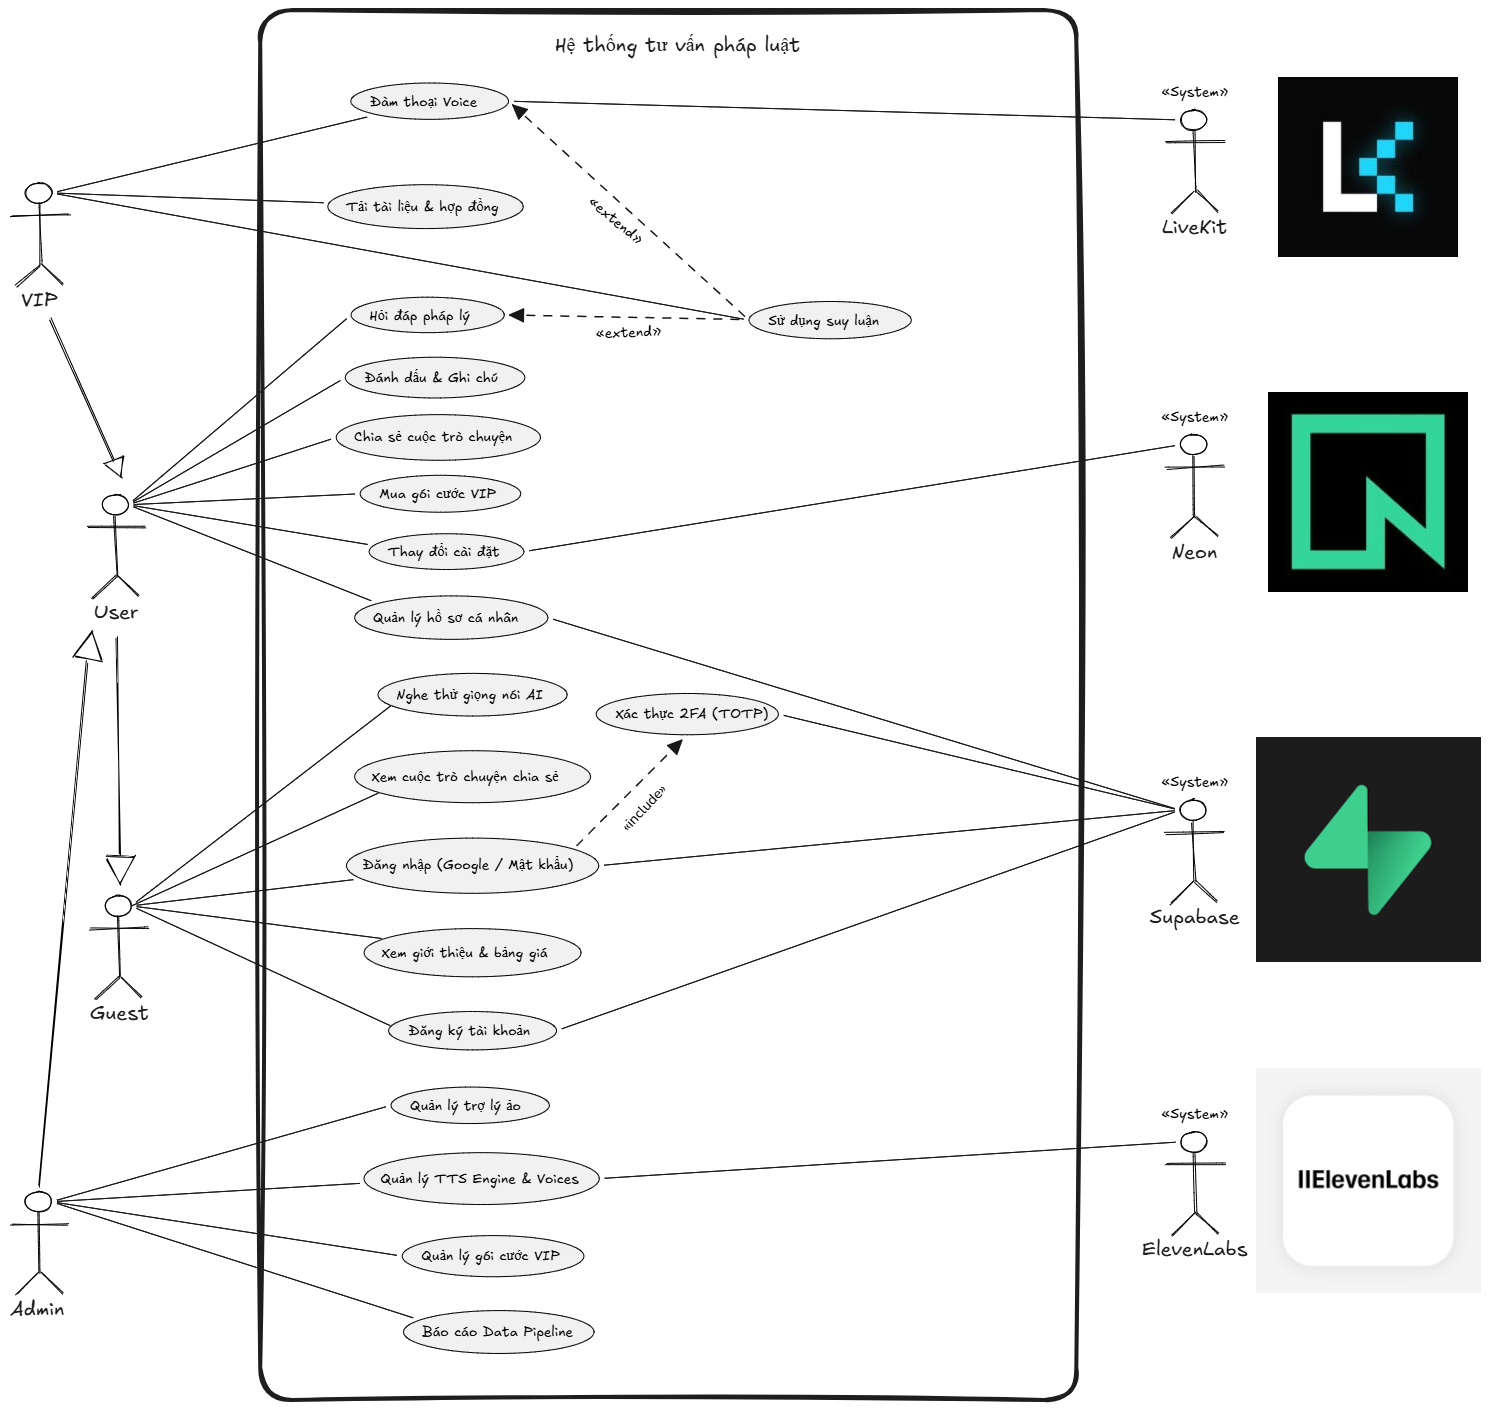
\includegraphics[scale = 0.18]{pictures/UseCase.excalidraw.png}
\caption{Sơ đồ Use Case}
\end{figure}


Hệ thống phân chia người dùng thành 4 nhóm đối tượng chính với các đặc quyền được kế thừa và mở rộng dần theo cấp độ:

\begin{itemize}

\item Khách vãng lai (Guest):
\begin{itemize}

\item Đặc điểm: Là những người dùng chưa có tài khoản hoặc chưa đăng nhập vào hệ thống. Mục đích chính của họ là tìm hiểu thông tin cơ bản về ứng dụng và trải nghiệm thử các tính năng công khai.

\item Quyền hạn: Có thể xem các trang giới thiệu, bảng giá gói cước; nghe thử các mẫu giọng nói của các nhân vật; xem các đoạn trò chuyện tư vấn pháp luật được người dùng khác chia sẻ công khai. Họ có thể thực hiện đăng ký tài khoản mới hoặc đăng nhập (qua email hoặc Google).

\end{itemize}

\item Người dùng phổ thông (User):
\begin{itemize}

\item Đặc điểm: Là những cá nhân đã đăng ký và đăng nhập thành công vào hệ thống. Đây là tệp khách hàng tiêu chuẩn sử dụng các tính năng hỏi đáp pháp lý cơ bản bằng văn bản. Tác nhân này kế thừa toàn bộ quyền của Guest.

\item Quyền hạn: Có thể chat/hỏi đáp pháp lý cơ bản với AI; sử dụng các công cụ cá nhân hóa như đánh dấu (bookmark), tạo ghi chú, thay đổi cài đặt và quản lý hồ sơ cá nhân. Người dùng có thể chia sẻ cuộc trò chuyện của mình cho người khác, bảo mật tài khoản bằng xác thực 2 lớp (2FA/TOTP) và có thể thực hiện nâng cấp/mua gói cước VIP.

\end{itemize}

\item Người dùng VIP (VIP):
\begin{itemize}

\item Đặc điểm: Là những người dùng đã thanh toán và đăng ký gói cước VIP. Họ có nhu cầu giải quyết các vấn đề pháp lý phức tạp, cần phân tích tài liệu chuyên sâu hoặc muốn tương tác rảnh tay qua giọng nói. Tác nhân này kế thừa toàn bộ quyền của User.

\item Quyền hạn: Được sử dụng các tính năng cao cấp bao gồm: Đàm thoại trực tiếp với AI bằng giọng nói (Voice chat qua LiveKit); tải lên các tài liệu, hợp đồng cá nhân để AI phân tích; và được phép sử dụng các mô hình suy luận (reasoning) nâng cao để giải quyết các truy vấn pháp lý phức tạp (áp dụng cho cả chat văn bản và đàm thoại).

\end{itemize}
\newpage
\item Quản trị viên (Admin):
\begin{itemize}

\item Đặc điểm: Là nhân sự thuộc ban quản trị/vận hành hệ thống. Họ có kiến thức về quản lý hệ thống, theo dõi luồng dữ liệu (Data Pipeline) và cấu hình các dịch vụ tích hợp giọng nói. Tác nhân này kế thừa toàn bộ quyền cơ bản của User.

\item Quyền hạn: Có toàn quyền truy cập trang quản trị để: Quản lý các nhân vật trợ lý ảo; thiết lập và quản lý hệ thống chuyển đổi văn bản thành giọng nói (TTS Engine và Voices kết nối với ElevenLabs); quản lý các gói cước VIP; và xem/theo dõi các báo cáo về luồng xử lý dữ liệu pháp luật (Data Pipeline).

\end{itemize}
\end{itemize}


\subsubsection{Sơ đồ tuần tự (Sequence Diagram)}


\subsection{Kiến trúc hệ thống}
\lipsum[1]
\subsection{Đường ống dữ liệu}
\lipsum[1]
